\documentclass[conference]{IEEEtran}
\usepackage{amsmath,amssymb,amsfonts}
\usepackage{algorithmic}
\usepackage{graphicx}
\usepackage{textcomp}
\usepackage{xcolor}
\usepackage{biblatex}
\usepackage{titlesec}
\usepackage{float}
\usepackage{listings,xcolor}


\def\BibTeX{{\rm B\kern-.05em{\sc i\kern-.025em b}\kern-.08em
		T\kern-.1667em\lower.7ex\hbox{E}\kern-.125emX}}


\addbibresource{references.bib}


\begin{document}
	
	\title{Interactive book system}
	
	\author{\IEEEauthorblockN{Carmel Gafa}
		\date{December 2024}
	}
	
	\maketitle
	
	\begin{abstract}
		This project presents an AI-powered storytelling platform designed to create interactive and engaging, story experiences for readers. The platform's design allows seamless integration of various AI components, providing a scalable solution for creative content generation. This work highlights AI's transformative potential in education and entertainment, offering an interesting approach to interactive storytelling.
	\end{abstract}
	
	\begin{IEEEkeywords}
		Interactive Storytelling, AI Content Generation, OpenAI GPT, Azure Text-to-Speech, React, Flask, Multi-Modal Applications, Educational Technology.
	\end{IEEEkeywords}
	
	\section{Introduction}
	
	Interactive storytelling systems have been a popular medium for delivering immersive and personalised experiences since the early days of home computing. In those early days, a genre of computer games emerged as text-based adventure games, where the story evolved based on user input through textual commands\cite{brooker2021filling}\cite{woodcock2012zx}. However, as computing power and graphical capabilities improved, the popularity of these games waned in favour of visually rich gaming experiences. Despite this decline, these games are still fondly remembered for their creativity and ability to engage.
		
	\begin{figure}[!h]
		\centering
		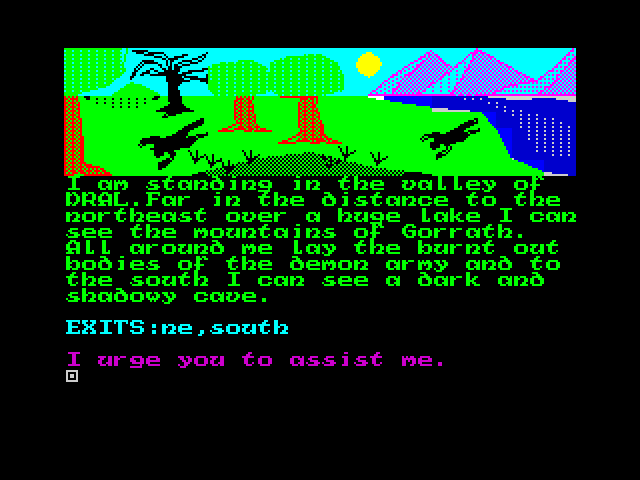
\includegraphics[width=0.7\linewidth]{img/img-ari3333-project-report-adventure-games}
		\caption{Demon from the Darkside was released in 1986 by Compass Software for ZX Spectrum 48K\cite{demonfromdarkside2020}}
		\label{fig:img-ari3333-project-report-adventure-games}
	\end{figure}
		
	Generative AI systems have the potential to introduce an innovative twist to stories by evolving based on user interaction\cite{vidrih2023generative} \cite{fotedar2020storytelling}. These technologies enable stories to adapt their plots in real time to align with the player’s mood and style.
	
	This paper takes a step in this direction by introducing an interactive book system—a web-based single-page application designed to ensure smooth, dynamic, and seamless user interaction. The system demonstrates the potential of Generative AI to provide engaging content that adapts to the user's age and taste, with these variables configured as system parameters.
	
	This paper is organised into the following sections:
	
	\begin{itemize}
		
		\item Section 2 examines the system, its outputs, and navigation.
		\item Section 3 discusses the system architecture.
		\item Section 4 looks st the system's workflows.
		\item Section 5 addresses the ethical considerations associated with such systems.
		\item Section 6 talks about the use of generative AI platforms that were used during the development of this application.
		
	\end{itemize}
	
	
	\section{The interactive book}
	
	The interactive book system is accessible through a web browser and features a user-friendly interface to ensure readers' engaging experience.
	
	Upon startup, the system displays the book's title page, which contains the book's name and a picture graphically aligned with the story's title, theme, and mood. The title page also contains a "start" button, which initiates the storytelling experience when pressed.
	
	The story will continue on the following pages, each with a segment of the story. Each page includes a speaker icon in the upper right corner, enabling a narration service to read the text to a user. This feature uses text-to-speech technology to benefit users who need or want audio output.
	
	Every page of the story also presents two choices for users through buttons that trigger the storytelling in a particular direction. Selecting one of them influences the drama of the unfolding story, making the adventure interactive and attractive. At the end of the story, no more extended options are available, but the user can start a new story. If the user selects that option, the system resets to the title page of a newly created story.
	
	Some examples of typical title and content pages that also include title images can be seen in Appendix \ref{appendix:navigation}.
	
	Controlling all stories are four variables. Adjusting these parameters allows the system to produce entirely different stories, making the interactive book adaptable to diverse audiences and contexts. 
	
	\begin{itemize}[]
		\item Reader's Age: This parameter defines the book's target readership.
		\item Theme of the Book: Defines the specific theme and mood of the book and can harness personal customisation to suit user preference.
		\item Author Style: This is an author's name that will affect the book's tone, diction, and narrative structure.
		\item Number of Pages: This will determine the number of pages in the story.
	\end{itemize}
	
	Different stories suited to diverse audiences and contexts were successfully generated by changing these parameters. When writing this document, these parameters can be modified as code arguments, but this task can be done quickly enough to export it to a user interface as settings.
	
	
	\section {System architecture}
	
	The system utilises a three-tier architecture, with backend generative AI services and text-to-speech features coordinated by a middle layer that manages prompting and result aggregation. A frontend layer supports user interaction and displays the book's text and images. Communication among the layers occurs through RESTful APIs, which maintain a clear separation of concerns. This separation improves maintainability and scalability, allowing future expansions and integrations to be carried out quickly.
	
	The backend application is implemented as a Python Flask application that serves as the core orchestrator for content generation and coordination. This layer integrates external APIs, including OpenAI GPT for text and image generation and Azure Cognitive Services for text-to-speech conversion, to deliver a multimodal storytelling experience. The architecture implemented in this exercise also abstracts the story parameters, prompts, and system keys into separate modules to easily extend and maintain the system.
	
	The frontend application is developed using React, leveraging its component-based architecture to ensure a user-friendly and visually engaging interface. As a single-page application, the system eliminates unnecessary page reloads, allowing users to navigate the story seamlessly while maintaining a dynamic and interactive experience. The frontend application also includes error-handling mechanisms to manage scenarios such as backend unavailability or invalid responses. Users are notified of such errors through messages in the user interface.
	
	A diagrammatic representation of the concepts discussed in this section is found in the system architecture diagram in Appendix \ref{appendix:system-architecture}
	
	\subsection{Interfaces and external dependencies}
	
	The backend system interacts with two services that provide large-language-model, image generation and speech capabilities:
	
	\begin{itemize}
		\item The OpenAI ChatGPT API generates the book title, individual page content, and the image used on the title page.
		\item The Azure Cognitive Services (Text-to-Speech) converts story content into audio files, allowing users to engage with the narrative audibly. This capability enhances accessibility and also provides an increased multi-modal user experience. The audio files are placed in a local folder and must be served to the front-end layer for consumption.
	\end{itemize}
	
	\subsection{The backend system}
	
	As described previously, the backend system of the interactive book manages the flow of data and communication between the front end, external APIs, and internal resources. The layer is organised to introduce additional functionality without changing its underlying structure. The following aspects were taken into consideration when designing this layer.
		
	\begin{enumerate}
		\item Integrations with large language models and text-to-speech systems are abstracted into specialised classes that provide a specific contribution to the interactive book, such as the book's writing, the image generation or the creation of the book image. These classes handle the integration with these engines and the management of message prompt arrays responsible for maintaining the context of a given interaction, which, in this case, is the evolution of the book.
		\item Prompt management was abstracted into a separate module so that each integration class would call this module to inject prompts into its respective system. This decision was made to maintain consistency between the various prompts and make prompt management easier. It is safe to assume that in producing systems with similar integrations, prompt creation and management are carried out by different teams, and prompts will be contained in specialised databases. The decision to abstract prompts is a step in this direction.
		\item As explained previously, all books are based on four parameters: the theme, the author's style, the target audience's age, and the desired number of pages. These parameters are also contained in a separate module, so the interactive book type can be changed quickly without changing any code.
		\item Flask API endpoints are the topmost level of this architecture and provide the most generic creation capabilities that, in most cases, consume some lower-level services. Such services include the creation of a title page or the creation of a page. The results of the endpoints are provided as JSON objects to the consumers
	\end{enumerate}
	
	\begin{figure}[H]
		\centering
		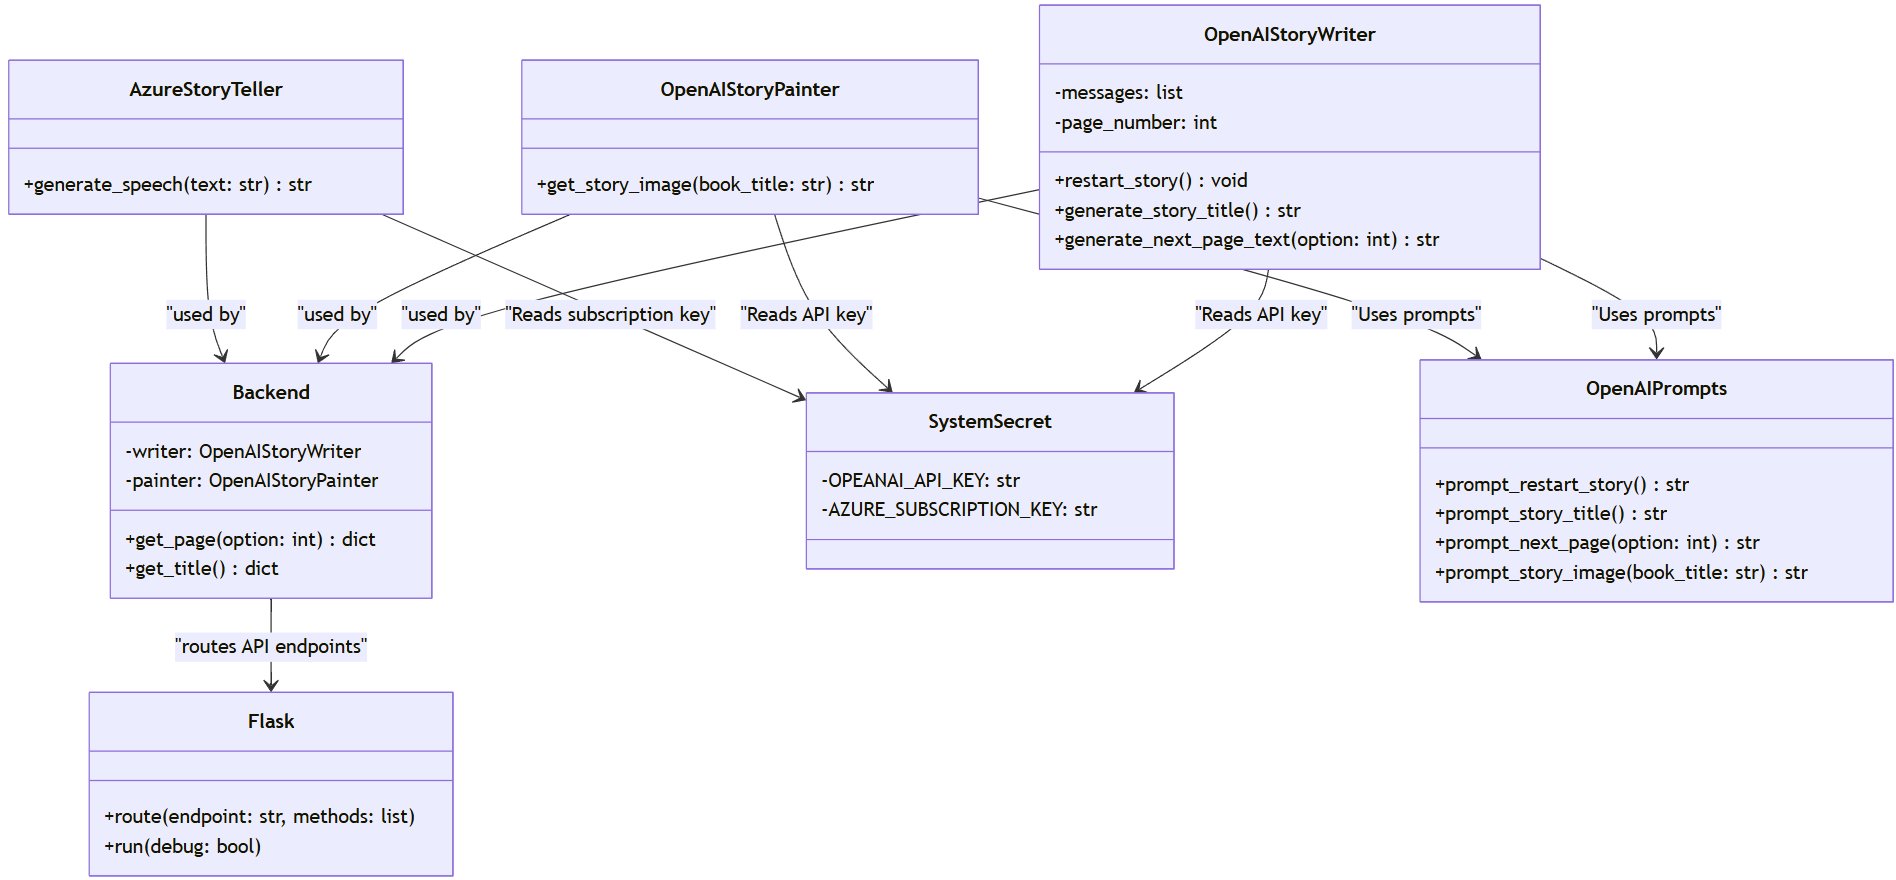
\includegraphics[width=0.9\linewidth]{img/img-ARI3333-backend-class-diagram}
		\caption{The interactive book backend system class diagram}
		\label{fig:img-ari3333-backend-class-diagram}
	\end{figure}
	
	\subsubsection{AI integration classes}
	
	This layer comprises three classes, each focusing on a specific interaction with OpenAI and Azure text-to-speech engines.
	
	\begin{enumerate}
		\item \textbf{\texttt{OpenAIStoryWriter}} creates the story's narrative using OpenAI's \textbf{\texttt{gpt-3.5-turbo}} engine. The class maintains a list of messages submitted and returned from the engine required to maintain context for a book being developed and the number of pages generated for a developing book. It has three main methods:
		\begin{itemize}
			\item\textbf{\texttt{restart\_story}} starts a new story by starting a new message array to be used with OpenAI and posting a first prompt that informs the engine about the theme, author style, target age and desired number of pages for the book to be generated.
			\item\textbf{\texttt{generate\_story\_title}} adds the book title creation prompt to the OpenAI message array and submits the message thread to the engine. The engine, in turn, returns the name of the new book.
			\item\textbf{\texttt{generate\_next\_page\_text}} generates a new page for the interactive book given a prompt.
		\end{itemize}
		\item\textbf{\texttt{OpenAIStoryPainter}} creates the story's title page image using OpenAI's image creation capabilities. This class does not maintain any context as it is only used to create an image based on very little information, namely the book's title. It has only one method:
		\begin{itemize}
			\item\textbf{\texttt{get\_story\_image}} generates a 256 by 256-pixel image based on the book's title.
		\end{itemize}
		\item\textbf{\texttt{AzureAIStoryTeller}} uses Microsoft Azure's cognitive services text-to-speech capabilities to generate an audio version of a page, including the options. The class has only one method:
		\begin{itemize}
			\item\textbf{\texttt{generate\_speech}} connects to Azure's text-to-speech service, providing the text for which the audio will be generated and the location where the resulting audio file should be stored. The method maps the file to a served URL, allowing any system to access the generated audio file.
		\end{itemize}
	\end{enumerate}
	
	\subsubsection{Secrets Storage}
	The backend manages all sensitive information, such as API keys and authentication tokens, through the Secrets Storage module. By isolating and protecting these credentials, the system maintains secure and reliable connections to external services and mitigates potential vulnerabilities. 
	
	\subsubsection{Story parameters}
	This module contains the four parameters required to create a book. Parameter management is an essential aspect of dynamic systems, such as interactive books, to ensure that the nature of the artefact produced can be easily adapted and extended. Although the abstraction system used in this project is trivial, it is also quite powerful, as the few parameters contained in this file can be modified to generate books with entirely different styles and themes.
		
	\subsubsection{Prompt management}
	The prompt management module contains prompts for components in the backend to generate the interactive book. It utilises the story parameters module to ensure consistency and relevancy in the book creation process. 
	
	Commercial projects that rely on generative AI systems depend on teams of specialised prompt engineers who will maintain their work in databases that the application uses as required. Abstracting prompts from the codebase is, therefore, an important step in such systems to ensure that multidisciplinary teams can work together,
	
	The table in Appendix D contains all the prompts used in this system.
		
	\subsubsection{API Interface}
	
	The API layer provides the interfaces so systems can consume the backend layer. As explained previously, it is written in Flask and contains just two endpoints:
	
	\begin{itemize}
		\item \textbf{\texttt{/API/title}} is the narrative's entry point. This call will instruct an \textbf{\texttt{OpenAIStoryWriter}} instance to generate a story title and an \textbf{\texttt{OpenAIStoryPainter}} instance to create a story image. It will, in turn, return an object with the following information:
		\begin{tabular}{ll}
			& \\
			\{& \\
			\textbf{\texttt{"title"}}: & \textbf{\texttt{"book\_title"}},\\
			\textbf{\texttt{"image\_url"}}& \textbf{\texttt{"image\_url"}}\\
			\}& \\
			& \\
		\end{tabular}

		\item \textbf{\texttt{/API/page/int: option}} is called to create a new page for the story, supplying the user-selected option. This call first instructs the \textbf{\texttt{OpenAIStoryWriter}} instance to generate the new page. The writer returns a string containing the information for the new page: the image text, the page options, and whether the story is completed. The page text and options are then formatted and supplied to an \textbf{\texttt{AzureAIStoryTeller}} instance to convert the text into speech. This interaction returns the location of the audio file in a URL that external systems can access. The information is then bundled into one object and returned.
	
		\begin{tabular}{ll}
			& \\
			\{& \\
			\textbf{\texttt{"part"}}: \textbf{\texttt{"The next part of the story"}},\\
			\textbf{\texttt{"option1"}}: \textbf{\texttt{"Option 1"}},\\
			\textbf{\texttt{"option2"}}: \textbf{\texttt{"Option 2"}},\\
			\textbf{\texttt{"status"}}: \textbf{\texttt{"Status"}},\\
			\textbf{\texttt{"textURL"}}: \textbf{\texttt{"URL of the aud file for page"}}\\
			\}& \\
			& \\
		\end{tabular}
	\end{itemize}
	
	\subsection{The frontend system}
	
	The interactive book system's front end is designed to deliver an engaging user experience. It is built using ReactJS as a single-page application that communicates with the backend tier to retrieve the dynamic content. The following sections discuss the frontend tier's components and workflows in more detail.
	
	At the core of the frontend tier is the \textbf{\texttt{Book}} component, which serves as the interactive interface through which the user interacts with the book's content. The book component has two modes of display:
	
	\begin{itemize}
		\item Title Page Display: If the book is at its starting point (page number = 0), the component retrieves and renders the book's title and the associated title image provided by the backend.
		\item Page Content Display: For all subsequent pages, the component displays the text content of the current page along with any user-selectable options for advancing the story.
	\end{itemize}
	
	In addition, this component monitors the story status for changes and re-renders to reflect the latest content retrieved from the backend. The status is particularly important when the last page of the interactive book is reached, as the book component will not display any options but prompts the user to start a new book
	
	The frontend also streams audio content from the backend tier, which, as explained previously, is generated using Azure Cognitive Services. The speech functionality seamlessly integrates into the user interface, enabling easy playback and pausing.
	
	
	\section{System Workflows}
	
	This section will discuss how the backend and frontend systems are integrated and coordinated so that the interactive book can function correctly. It also illustrates the synchronization process between text, image, and audio generation to ensure all modalities align seamlessly.
	
	\subsection{Initial Page Loading}
	
	When the application is first launched, the frontend performs the following tasks, as shown in Figure \ref{fig:img-ari3333-loading-workflow}:
	
	\begin{enumerate}[]
		\item API Call to the backend system: The frontend system requests the backend \textbf{\texttt{api/title}} endpoint to retrieve the book's title and the associated title image.
		\item Rendering the Title Page: Upon receiving the response, the Book component displays the title text and image on the screen. The user is then prompted to proceed to the story's first page.
	\item \end{enumerate}
	
	\begin{figure}[H]
		\centering
		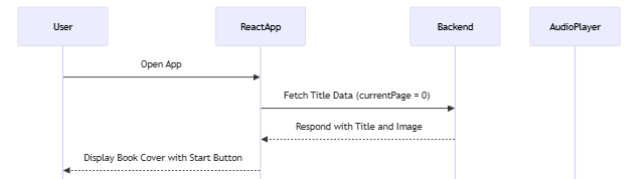
\includegraphics[width=0.9\linewidth]{img/img-ARI3333-loading-workflow}
		\caption{Interactive book loading workflow}
		\label{fig:img-ari3333-loading-workflow}
	\end{figure}
	
	When the user selects the Start button, the following tasks take place as can be seen in Figure \ref{fig:img-ari3333-initiation-workflow}:
	
	\begin{enumerate}[]
		\item API Call to Fetch the First Page: The frontend sends a \textbf{\texttt{GET}} request to the backend endpoint specifying that the selected option, in this case, is 0, as there was no option selection, \textbf{\texttt{/api/page/0}} to retrieve the first page's content, options, and associated audio file URL.
		\item Rendering the First Page: The Book component updates to display the text for the first page, the user-selectable options for advancing the story, and an audio playback button that can be used to play the generated speech.
	\end{enumerate}
	
	\begin{figure}[H]
		\centering
		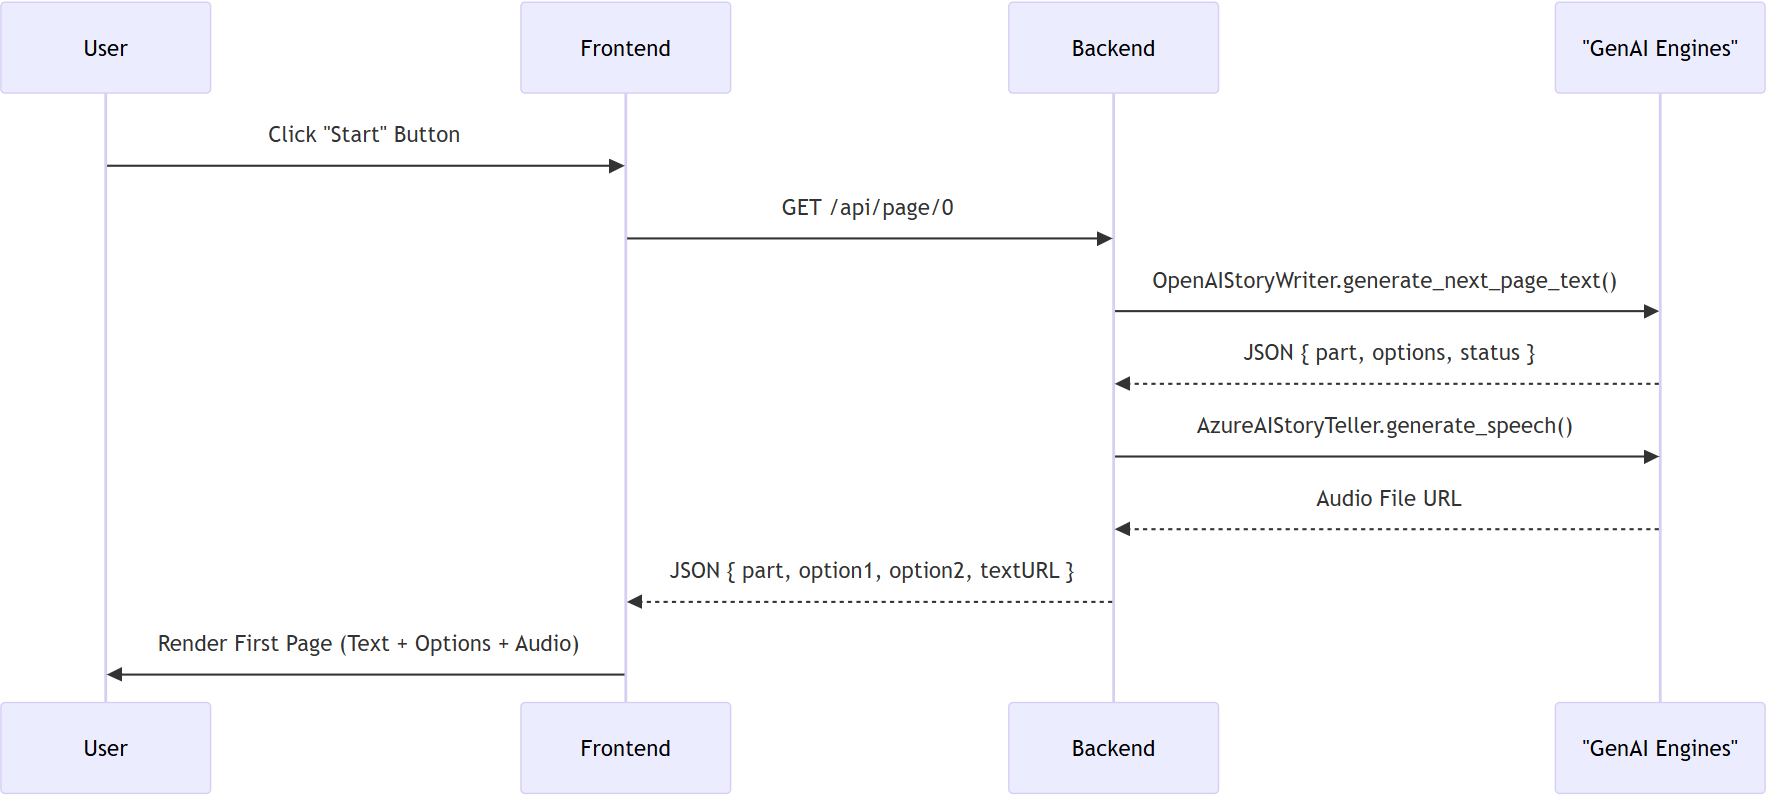
\includegraphics[width=0.7\linewidth]{img/img-ARI3333-initiation-workflow}
		\caption{Interactive book press Start button workflow}
		\label{fig:img-ari3333-initiation-workflow}
	\end{figure}
	
	\subsection{Page Navigation Workflow}
	
	The user progresses through the story by selecting options. The tasks that take place are very similar to those executed when the start button is pressed, as we can see in Figure \ref{fig:img-ari3333-navigation-workflow} but in this particular case, a valid option is specified and subsequently processed by the backend:

	\begin{enumerate}[]
		\item User action: The user clicks either option button to determine the story's next segment.
		\item Backend communication: The frontend system sends a request to the backend, providing details about the selected option number.
		\item Content rendering: The backend returns the text, audio URL, status and options for the next page. The \textbf{\texttt{Book}} component updates to display the new content.
	\end{enumerate}
	
	\begin{figure}[H]
		\centering
		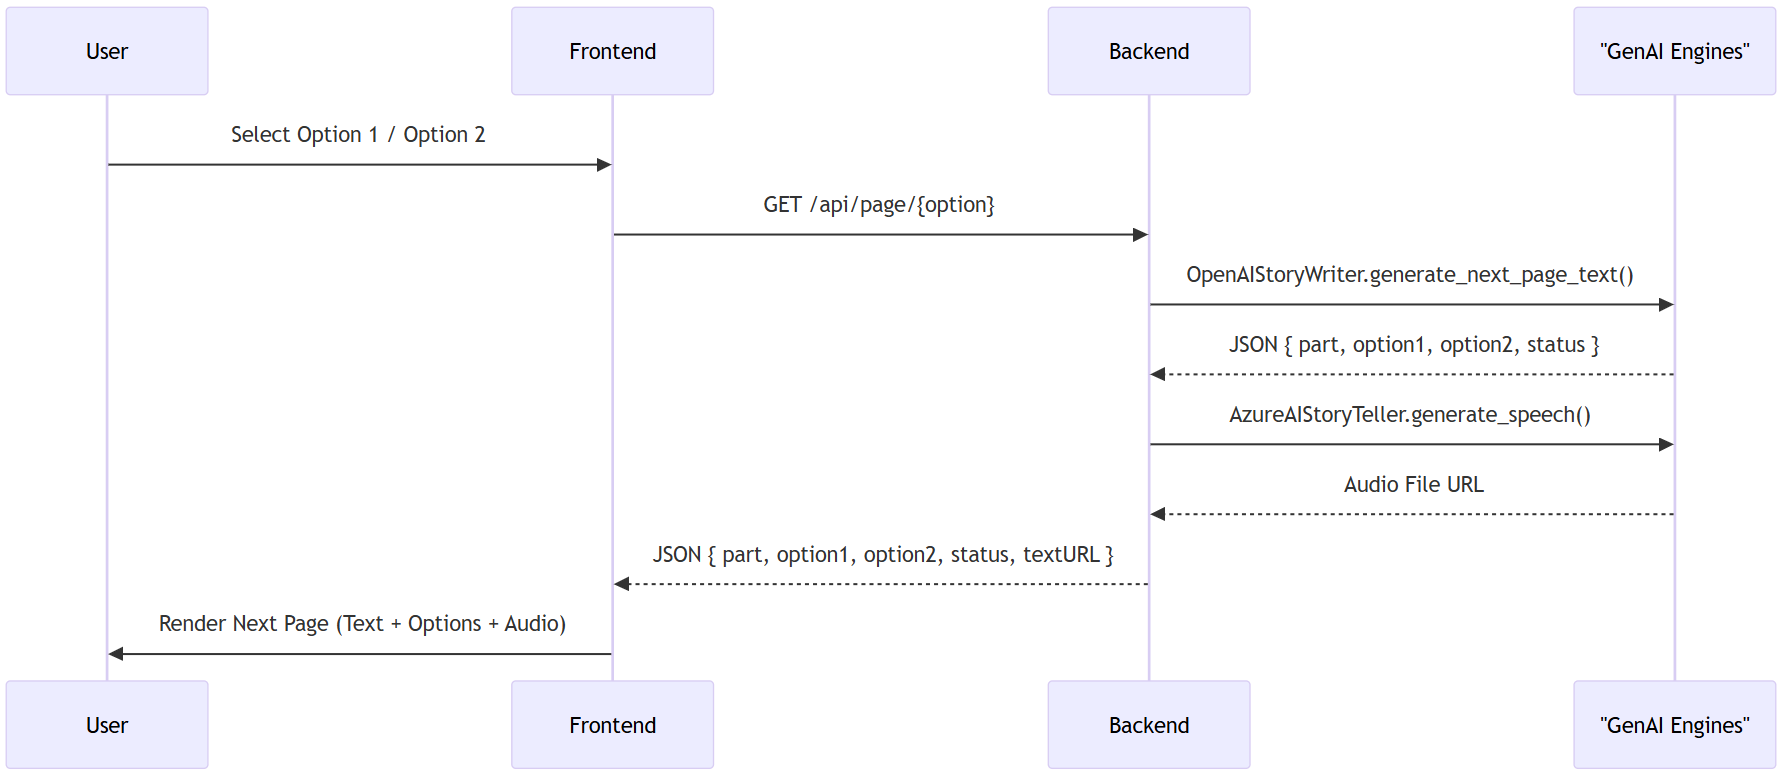
\includegraphics[width=0.7\linewidth]{img/img-ARI3333-navigation-workflow}
		\caption{Interactive book navigation workflow}
		\label{fig:img-ari3333-navigation-workflow}
	\end{figure}
	
	\subsection{Completion Workflow}
	
	Figure \ref{fig:img-ari3333-completion-workflow} similar sequence of events occurs when the end of the interactive book is reached. In this case, the status flag is set to complete, and the \textbf{\texttt{Book}} component in the frontend tier will not display the options and invite the user to start a new book instead. If selected, a reset action triggers a call to the backend, resetting the book's state and fetching a new title and initial page content.
	
	\begin{figure}[H]
		\centering
		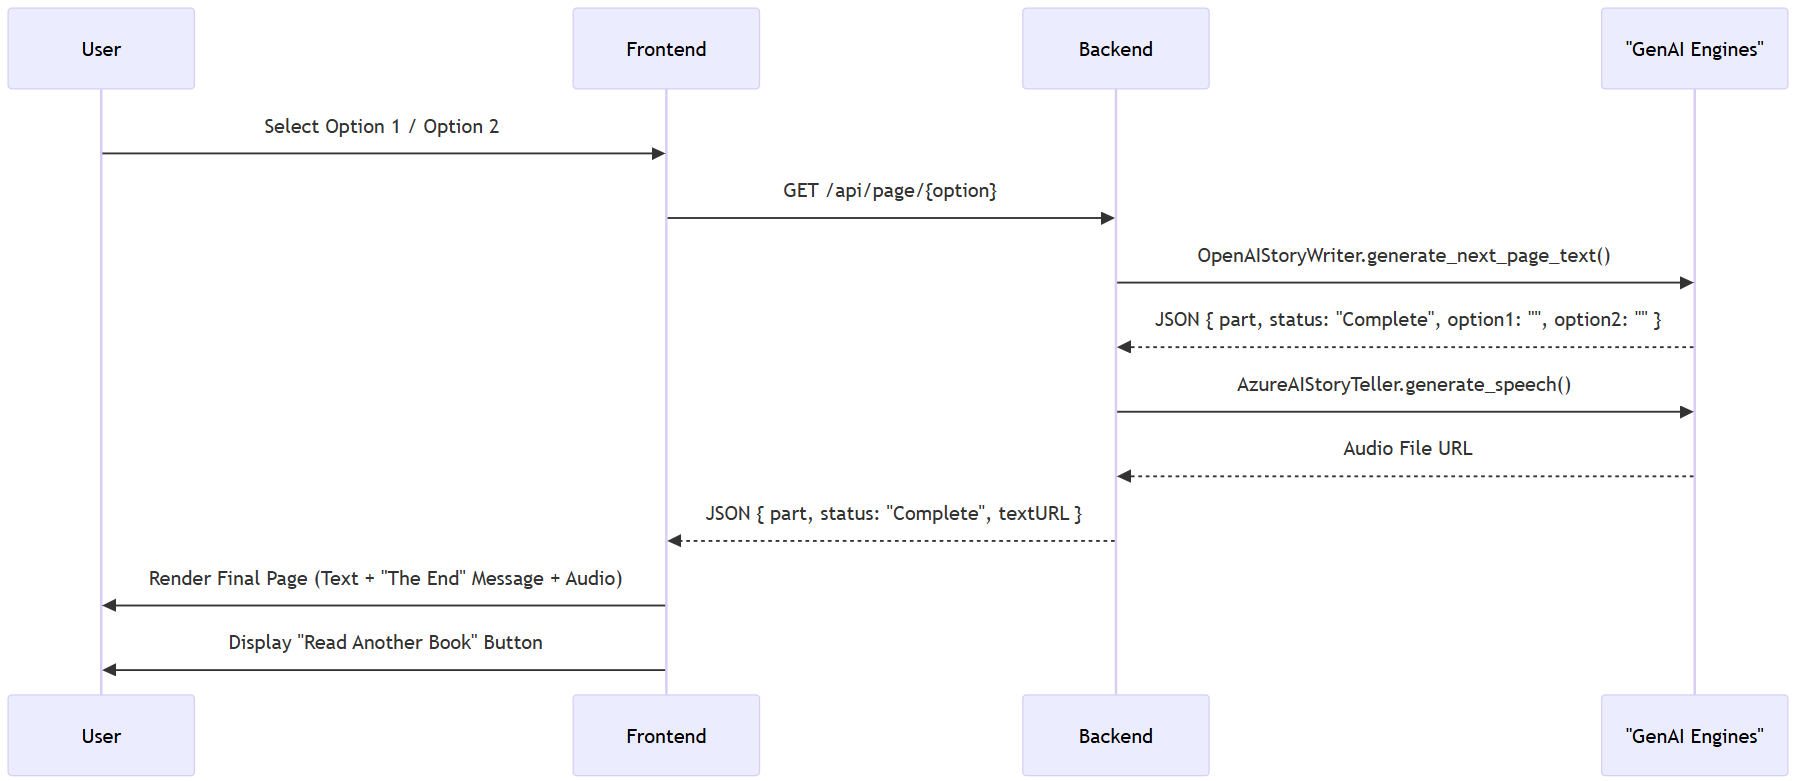
\includegraphics[width=0.7\linewidth]{img/img-ARI3333-completion-workflow}
		\caption{Interactive book completion workflow}
		\label{fig:img-ari3333-completion-workflow}
	\end{figure}
	
	
	\section{Ethical considerations}
		
	The previous sections show how an interactive book system can be constructed using popular technologies. The system is also reasonably easy to develop and extend. However, many social and ethical considerations surround AI-generated interactive books. The considerations have profound implications that extend beyond literature and technology. In this section, we will mention some of these considerations and discuss why the realization of such systems is so complex.
	
	There are concerns about the possible devaluation of human creativity if AI-generated content becomes popular. The increasing role of AI in creative processes, especially in the case of interactive storytelling, challenges traditional notions of authorship and human creativity \cite{udhayakumarexploring}. As AI systems become more sophisticated, it becomes essential to re-evaluate how we define and value human input in artistic endeavours. This shift in thinking could lead to new collaborative models between humans and AI, where both contribute to the creative process\cite{udhayakumarexploring}.
		
	AI-generated interactive books, by their nature, influence the readers, primarily if the stories are targeted at children\cite{salazar2024generative}. The nature of such stories is highly complex because the stories may not be repeatable and are unique in every generation.   If any of these narratives are biased or lack diversity, they risk perpetuating harmful stereotypes and reinforcing societal inequalities. Addressing bias in AI systems is therefore crucial to ensure that these forms of storytelling represent a wide range of voices and perspectives. The ethical development and deployment of AI in creative fields are essential to prevent the reinforcement of harmful ideologies through technology. In addition, if the readers feel that their choices are predetermined or that the AI is steering them towards specific outcomes, they will have their trust in the interactive experience eroded considerably, impacting their broader adoption and acceptance of AI-generated content. AI-generated interactive books have massive educational potential as they offer engaging and personalized learning experiences. Addressing bias, ensuring transparency, and fostering critical thinking skills in students is essential. 
	
	It is also crucial to avoid over-reliance on AI and ensure that these technologies enhance, rather than replace, human educators\cite{salazar2024generative}. Educators are already raising concerns about plagiarism and the academic integrity of AI tools. Studies\cite{delello2023exploring} highlight the increasing use of AI for assignments, with 43\% of college students admitting to using AI like ChatGPT for schoolwork, raising difficult questions about what constitutes cheating and how to assess student work fairly.
	
	Instructors may also be tempted to rely on AI writing assistants to ease their workload. However, if these tools are biased, they could lead to unfair grading practices, as one study illustrated in a hypothetical scenario where AI feedback disproportionately focuses on grammar for minority students while suggesting content ideas for others\cite{salazar2024generative}.
	
	Another interesting aspect of such systems is the balance between personalization and privacy\cite{kutty2021personalization}. Sophisticated personalization entails the collection and utilization of reader data, and this raises concerns about privacy and the potential misuse of personal information. Readers should have control over their data and be informed about how their information shapes their interactive experiences.
	
	The blurring of authorship lines and the collaboration between humans and AI necessitate a re-evaluation of existing legal frameworks, particularly regarding copyright and intellectual property rights\cite{kur2019european}. Determining ownership and attribution in AI-generated works presents legal challenges that require careful consideration. As AI plays a more significant role in creative industries, new legal and regulatory frameworks may be needed to address the unique challenges posed by these technologies.

	
	\section{Use of GenAI platforms in this project}
		
	Throughout this project, AI tools were used to validate and enhance the quality of the deliverables. The following outlines the tools employed and their impact on the development process:
	
	\begin{itemize}
		\item \textbf{\texttt{ChatGPT}} was utilized to enhance the quality of the styles for the frontend layer. Starting with an initial draft, iterative improvements were made to the look and feel of the interface through \textbf{\texttt{ChatGPT}} prompts, yielding excellent results. Additionally, all code produced during the project was reviewed using \textbf{\texttt{ChatGPT}} for validation and improvement. Many of the suggestions were deemed acceptable in the context of this project and subsequently implemented.
		
		\item This document was reviewed with \textbf{\texttt{Grammarly}} to identify and correct grammar errors, ensuring polished and professional writing.
		
		\item The ethical considerations section was developed with the help of \textbf{\texttt{ChatGPT}}, which helped create the keyword for the Scopus academic search engine. \textbf{\texttt{Elicit}} was also used, and good results were obtained in this phase. The papers that were identified were processed and managed in Google's \textbf{\texttt{NotebookLM}}.
	\end{itemize}
	
	Several key lessons emerged during the project:
	
	\begin{itemize}
		\item All the engines mentioned in this section are better suited when improving something already created. Asking any of these engines to produce something from scratch always resulted in a generic artefact unsuitable for a final deliverable..
		
		\item Code suggestions should be scrutinized before being implemented. Although many suggestions did improve the layout of the code for both the Python backend and the react frontend, there were also many suggestions that were plain wrong or relied on deprecated versions or modules. 
		
		\item A robust workflow that improves the inputs to work upon is vital. These inputs include papers and materials to help us quickly digest large amounts of data. The workflow used was \textbf{\texttt{Elicit}} for paper identification, \textbf{\texttt{NotebookLM}} for paper processing, and \textbf{\texttt{ChatGPT}} for validation.
	\end{itemize}


	\section{Conclusion}
	
	This project showcases how integrating modern AI technologies, such as OpenAI and Azure cognitive services, can deliver an interactive and engaging storytelling platform for young readers. By combining React for a dynamic single-page front-end, Flask for a robust backend, and these AI models for text, image, and speech generation, the system creates a sophisticated multi-modal user experience. 
	
	This work also highlights the potential of AI in creative content generation, emphasising simplicity, user interactivity, and age-appropriate narratives, serving as a foundation for future innovations in educational and entertainment applications.

	
	\section{Addendum - Inappropriate content filtering}
	
	An issue that was dealt with after this project was already in an advanced state was the question of content filtering. The interactive book application has been designed so that the reader's age is specified as one of the parameters driving all content creation efforts. However, implementing safeguards for such content, especially when children are involved, is paramount.
	
	For this reason, a simple but effective content-checking solution has been implemented in the \textbf{\texttt{OpenAIStoryWriter}} class using the \textbf{\texttt{profanityfilter library}}. \textbf{\texttt{Profanityfilter}} is an open-source Python library that detects and obfuscates profanity from the text and replaces such text with \textbf{\texttt{***}}.
	
	Although this solution is arguably simplistic, it provides a first level of protection to readers at the word level. It is obvious that additional levels need to be incorporated for similar commercial systems, but these will be implemented through a separate mechanism, such as profanityfilter.

	
\printbibliography
\onecolumn
\pagebreak

\appendices

\section{Story Navigation}
\label{appendix:navigation}
	
	\begin{figure}[H]
		\centering
		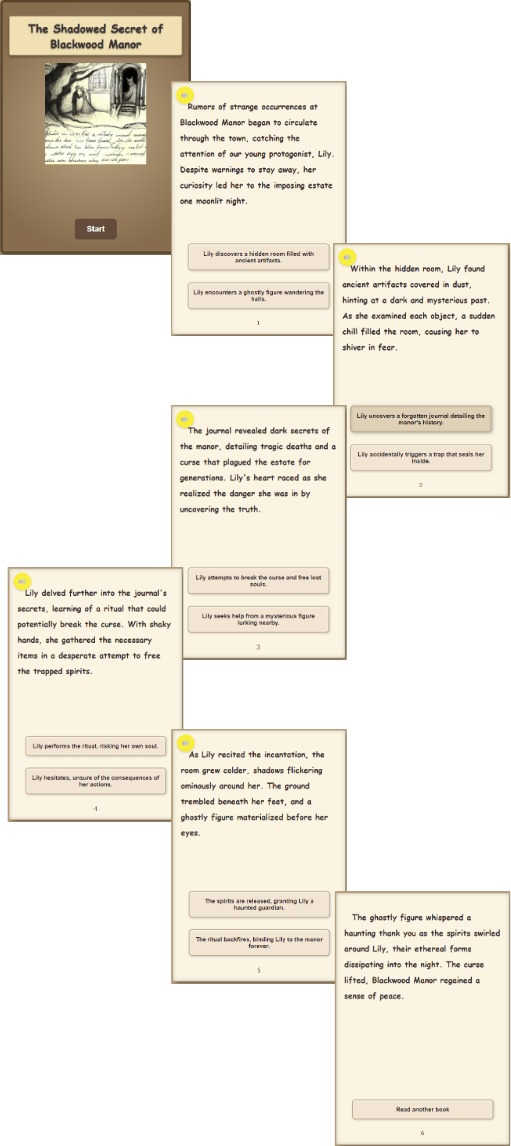
\includegraphics[width=0.5\linewidth]{img/img-ari3333-project-report-story-horror}
		\caption{Interactive book navigation for a horror story}
		\label{fig:img-ari3333-project-report-story-horror}
	\end{figure}
	
	\begin{figure}[H]
		\centering
		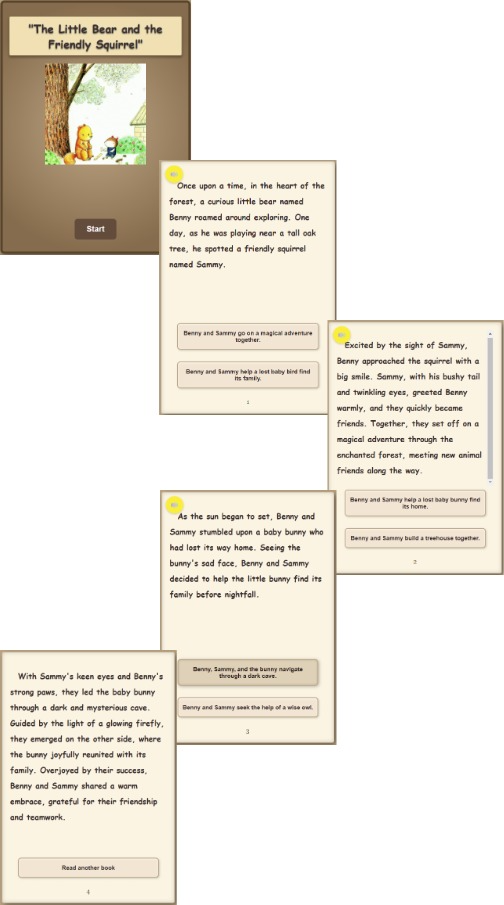
\includegraphics[width=0.7\linewidth]{img/img-ari3333-project-report-story-children}
		\caption{Interactive book navigation for a children's story}
		\label{fig:img-ari3333-project-report-story-children}
	\end{figure}

	
\pagebreak	
\section{System architecture diagram}
\label{appendix:system-architecture}

	\begin{figure}[H]
		\centering
		\includegraphics[width=0.9\linewidth]{"img/img-ARI3333-project-conceptual-diagram (1)"}
		\caption{Interactive book architecture diagram}
		\label{fig:img-ari3333-project-conceptual-diagram-1}
	\end{figure}


\pagebreak
\section{Interactive book prompts}

	\begin{table}[H]
	\centering
	\begin{tabular}{|l|p{8cm}|}
		\hline
		& \\
		\textbf{Prompt name} & \textbf{Prompt text} \\
		& \\ \hline
				
		& \\
		\textbf{\texttt{prompt\_restart\_story}} & You will create a story for a \textbf{\texttt{READER\_AGE}}-year-old using the style of \textbf{\texttt{BOOK\_STYLE}}. The story should have a simple structure with an introduction, a conflict, and a resolution. Each 'page' of the story should be two sentences long, except for the final page,which should contain only the words \textbf{\texttt{'The End'}} and nothing else. Make it engaging and age-appropriate but make sure that there is \textbf{\texttt{BOOK\_THEME}}.The story should be NOT MORE THAN \textbf{\texttt{MAXIMUM\_PAGES}} pages long. Introduce the main character of the story in the first page. \\ 
		& \\ \hline
		
		& \\
		\textbf{\texttt{prompt\_story\_title}} & Give me only the title of the story. \\
		& \\ \hline
		
		& \\
		\textbf{\texttt{prompt\_next\_page}} & Given that I selected option \textbf{\texttt{OPTION}}, give me the next part of the story in a paragraph that extend the story so far and on the option I selected.Give me also two possible ways to evolve the story, that should be not more than ten words; unless you are on the final page. In this case, the text will be \textbf{\texttt{'The End'}}. Label them \textbf{\texttt{'Option 1'}} and \textbf{\texttt{'Option 2'}}. Give me also a status for the story, which can be one of the following: \textbf{\texttt{'In Progress'}} or \textbf{\texttt{'Complete'}} .Package your reply in a JSON object with the following format: \textbf{\texttt{ \{"part": "The next part of the story", "option1": "Option 1", "option2": "Option 2", "status": "Status" \} }} \\
		& \\ \hline
				
		& \\
		\textbf{\texttt{prompt\_story\_image}} & A pencil-drawn illustration evoking a storybook atmosphere of \textbf{\texttt{BOOK\_THEME}}. The drawing style is aligned with the writing of \textbf{\texttt{BOOK\_STYLE}}. The title of the story is \textbf{\texttt{TITLE}} \\
		& \\ \hline
		
	\end{tabular}
\end{table}

	
\end{document}
